\chapter{Benutzerdokumentation}
\label{ch:4}

\section{Installation}
\subsection{Voraussetzungen und Installation der kompilierten Version}
F\"ur die Installation der Software ist ein Linux basiertes Betriebssystem notwendig. Die folgenden Schritte beschreiben den Installationsprozess f\"ur die bereits kompilierte Version. Diese Version wurde auf dem RWTH-Cluster sowie Ubuntu 14.04.3 LTS erfolgreich getestet.
\begin{enumerate}
  \item Entpacken des Archivs {\tt minimalflaechen\_projekt\_gruppe2.zip} in den gew\"unschten Installationsort.
  \item Wechseln in das Verzeichnis {\tt minimalflaechen\_projekt\_build}.
  \item Ausf\"uhren des Skripts {\tt minimalflaechen.sh} \"offnet das Programm. \\ \textit{Hinweis: Um das Skript ausf\"uhren zu k\"onnen m\"ussen gegebenenfalls Rechte f\"ur dieses mithilfe des Befehls {\tt chmod -x ./minimalflaechen.sh} gesetzt werden.}
\end{enumerate}

\subsection{Installation der unkompilierten Version}
Die unkompilierte Version des Programms findet sich in dem Verzeichnis {\tt minimalflaechen\_projekt\_source}. \"Offnen und konfigurieren des Projekts erfordert das Programm Qt Creator sowie die Installation der QT Bibliotheken. Zus\"atzlich dazu m\"ussen die Bibliotheken {\tt qwtplot3d} und {\tt matheval} kompiliert und in die Ordner {\tt libmatheval/lib} und {\tt qwtplot3d/lib} in dem Projektverzeichnis kopiert werden. Der Source-Code der Bibliotheken befindet sich in dem Verzeichnis {\tt ThirdParty}. Die Kompilierung dieser Bibliotheken ist unterschiedlich f\"ur verschiedene Betriebssysteme und erfordert ggf. weitere Bibliotheken. Bei Fragen bitte an {\tt stefan.jeske@rwth-aachen.de} wenden.

{\em wohlstrukturierte und gut lesbare Dokumentation basierend auf
den Anwendungsf\"allen}

\section{Speichern und Laden}
Die Applikation verf\"ugt \"uber eine Speicher- und Lade Funktionalit\"at. Die Einstellungen (Randfunktionen, numerische Parameter und Gebietsgr\"o\ss e) kann man in einem \textbf{.setup} Format und die berechnete Minimalfl\"ache kann man in einem \textbf{.surface} Format speichern und laden
%Evtl ein Bild vom Hauptfenster
\subsection{.setup-Format}
Das Speichern und Laden der Einstellungen arbeiten mit Dateien im \textbf{.setup}-Format.
Die Datei ist so aufgebaut, dass sich in jeder Zeile Informationen zu den eingegebenen Werten/Funktionen befinden, welche mit einem Semikolon am Ende abgetrennt werden. 
Dabei spielt die Reihenfolge der Informationen eine wichtige Rolle. Die Informationen von der ersten bis zur letzten Zeile:
\begin{enumerate}
\item epsilon - Genauigkeit der L\"osung
\item iterations - Maximale Iterationsschritte
\item n - Anzahl der St\"utzstellen in x-Richtung
\item m - Anzahl der St\"utzstellen in y-Richtung
\item xmin - untere x-Grenze
\item xmax - obere x-Grenze
\item ymin - untere y-Grenze
\item ymax - obere y-Grenze
\item a - Randfunktion auf der linken Seite des Gebietes
\item b - Randfunktion auf der oberen Seite des Gebietes
\item c - Randfunktion auf der rechten Seite des Gebietes
\item d - Randfunktion auf der unteren Seite des Gebietes
\end{enumerate}
%Bild Einstellungen_Speichern_2.png
\hfill \newline
\epsfig{file=nutzerdoc/Einstellung_Speichern_2.eps,width=\textwidth}
\subsection{.surface-Format}
Das Speichern und Laden der Einstellungen arbeiten mit Dateien im \textbf{.surface}-Format
Eine \textbf{.surface}-Datei ist in zwei Abschnitten aufgebaut. 
Im ersten Abschnitt enth\"alt die Datei ein paar grundlegende Informationen zu den Eingabedaten der Berechnung:
\begin{enumerate}
\item n - Anzahl der St\"utzstellen in x-Richtung
\item m - Anzahl der St\"utzstellen in y-Richtung
\item iterations - Maximale Iterationsschritte
\item epsilon - Genauigkeit der L\"osung
\item xmin - untere x-Grenze
\item xmax - obere x-Grenze
\item ymin - untere y-Grenze
\item ymax - obere y-Grenze
\end{enumerate}
Der zweite Abschnitt enth\"alt die berechnete Minimalfl\"ache inklusive den ausgewerteten R\"andern.
Jeder Wert wird mit einem Semikolon getrennt und insgesamt stellen die Zahlen die Eintr\"age von der Ergebnismatrix dar. (L\"osung von Ax=b, mit x als eine Matrix transformiert)

Hinweis: Die L\"osung der Minimalfl\"ache ist so gespeichert, dass man die Daten mit Programmen wie Excel oder Matlab weiterarbeiten kann. Die Semikolons dienen zur Trennung zwischen den einzelnen Daten, wie sie bei Excel z.B. mit unterschiedlichen Zellen realisiert werden.

\epsfig{file=nutzerdoc/surface_format.eps,width=\textwidth}

Nachdem der Nutzer den Button "'Einstellungen speichern" geklickt hat, erscheint ein Dialogfenster, wo der Nutzer den Speicherpfad, sowie den Dateinamen eingeben kann. Nach der Bet\"atigung des Save Buttons wird dann die Datei im \textbf{filename.setup} erstellt. 
\newline
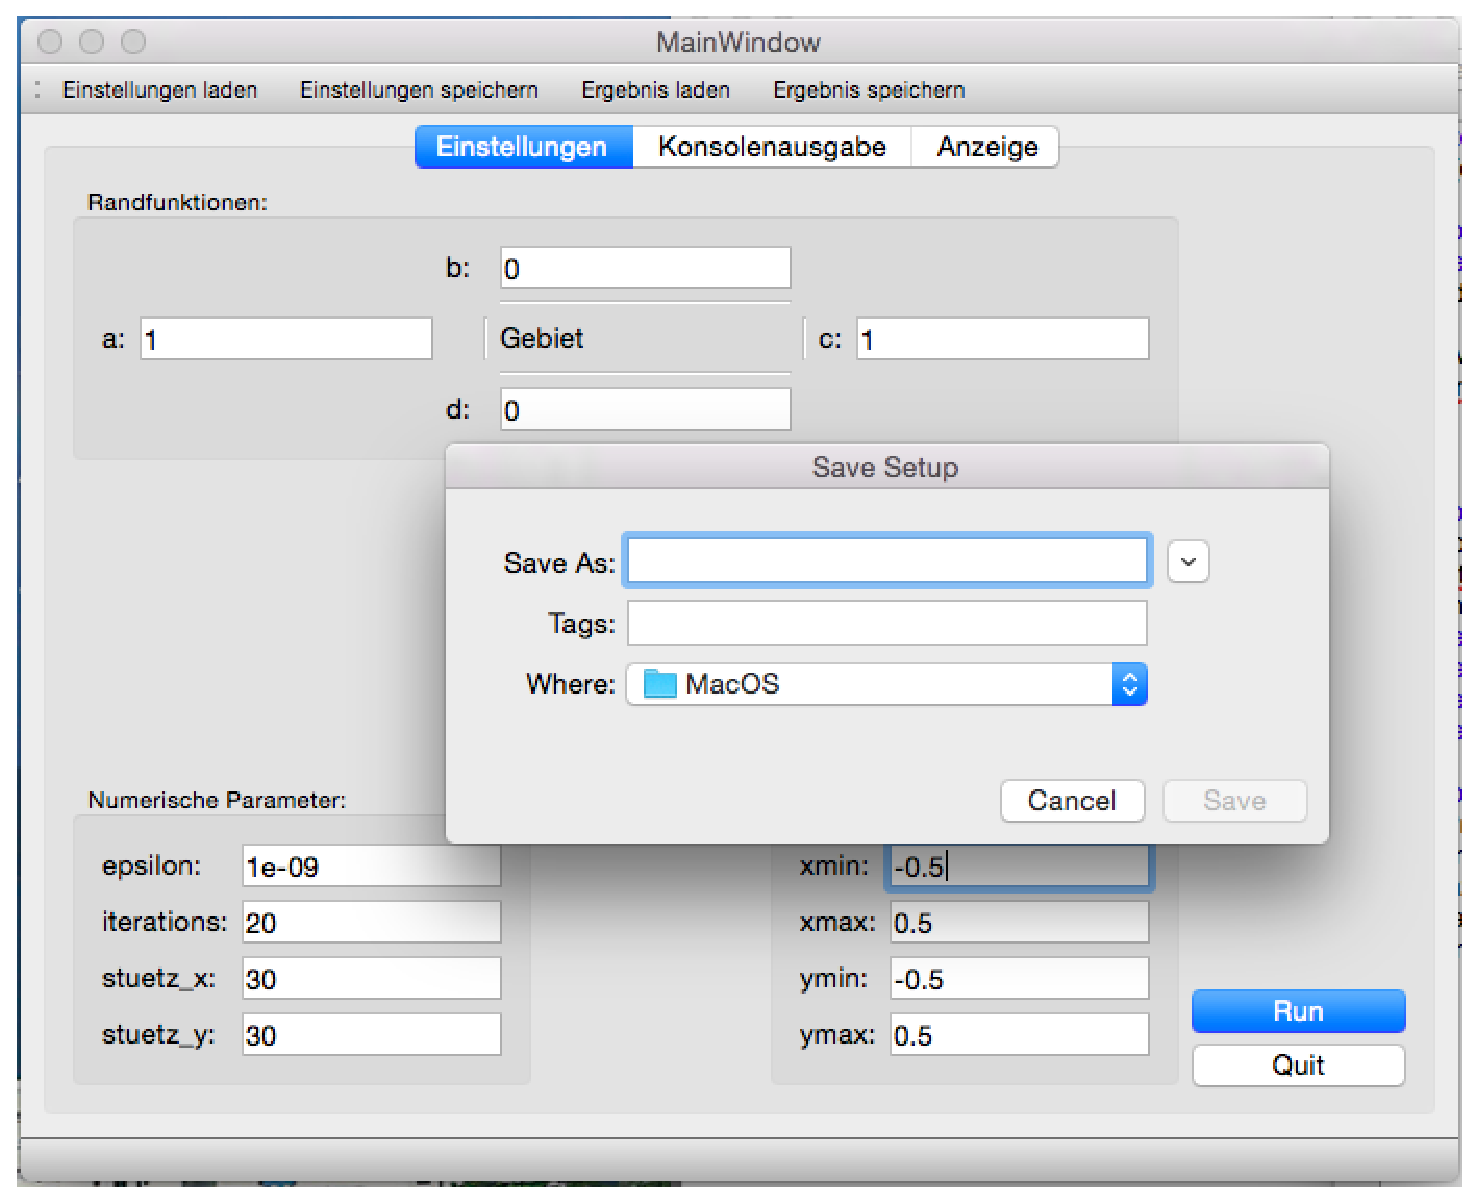
\epsfig{file=nutzerdoc/Einstellung_Speichern_1.eps,width=\textwidth}
% Bild Einstellungen_Speichern_1.png

\subsection{Einstellungen laden}
Nachdem der Nutzer den Button "'Einstellungen laden" geklickt hat, erscheint ein Dialogfenster, wo der Nutzer das Verzeichnis suchen kann, wo sich die Datei im \textbf{.setup}-Format befindet. Durch anschlie\ss endes Klicken auf den Open-Button werden die Randfunktionen, numerischen Parameter sowie die Gebietsgr\"o\ss e im Tab Einstellungen aktualisiert.
\newline
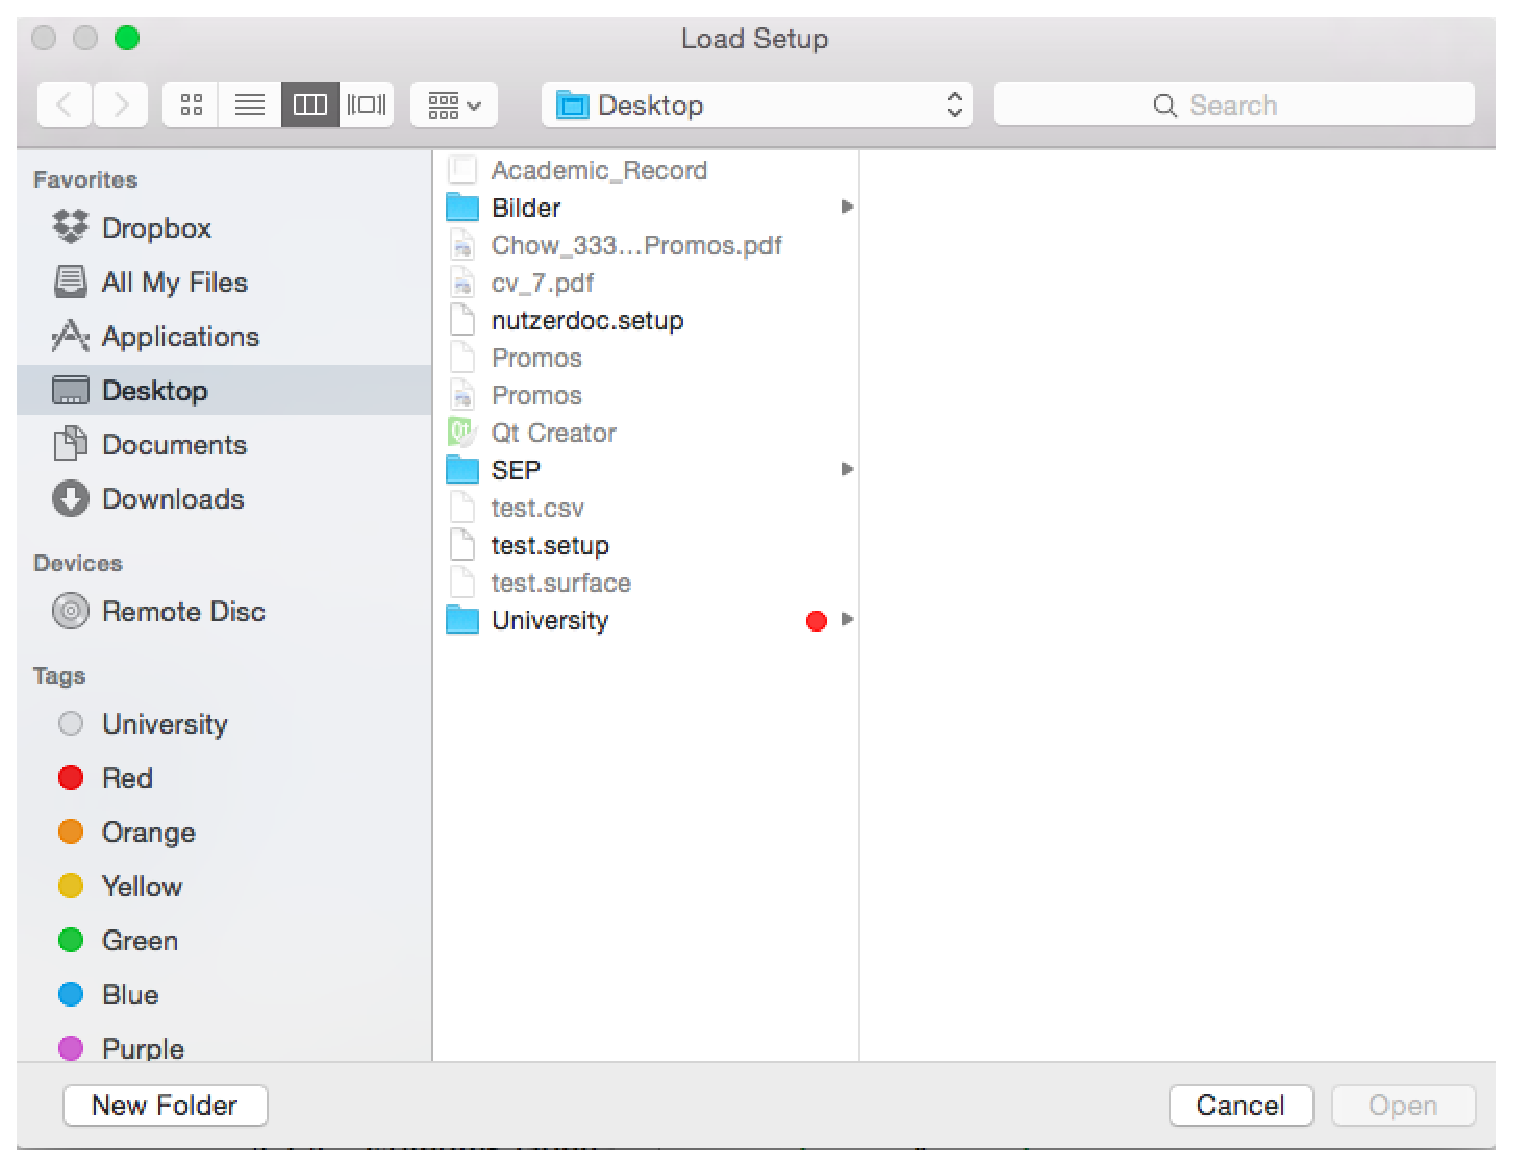
\epsfig{file=nutzerdoc/Einstellung_Laden_1.eps,width=\textwidth}

%Bild Einstellung_Laden_1.png
\subsection{Ergebnis speichern}
Nachdem der Nutzer den Button "'Ergebnis speichern" geklickt hat, erscheint ein Dialogfenster, wo der Nutzer den Speicherpfad, sowie den Dateinamen eingeben kann. Nach der Bet\"atigung des Savebuttons wird dann die Datei im \textbf{filename.surface} erstellt.
Hinweis: Speicherung eines Ergebnisses erst nach der Berechnung m\"oglich.
\newline
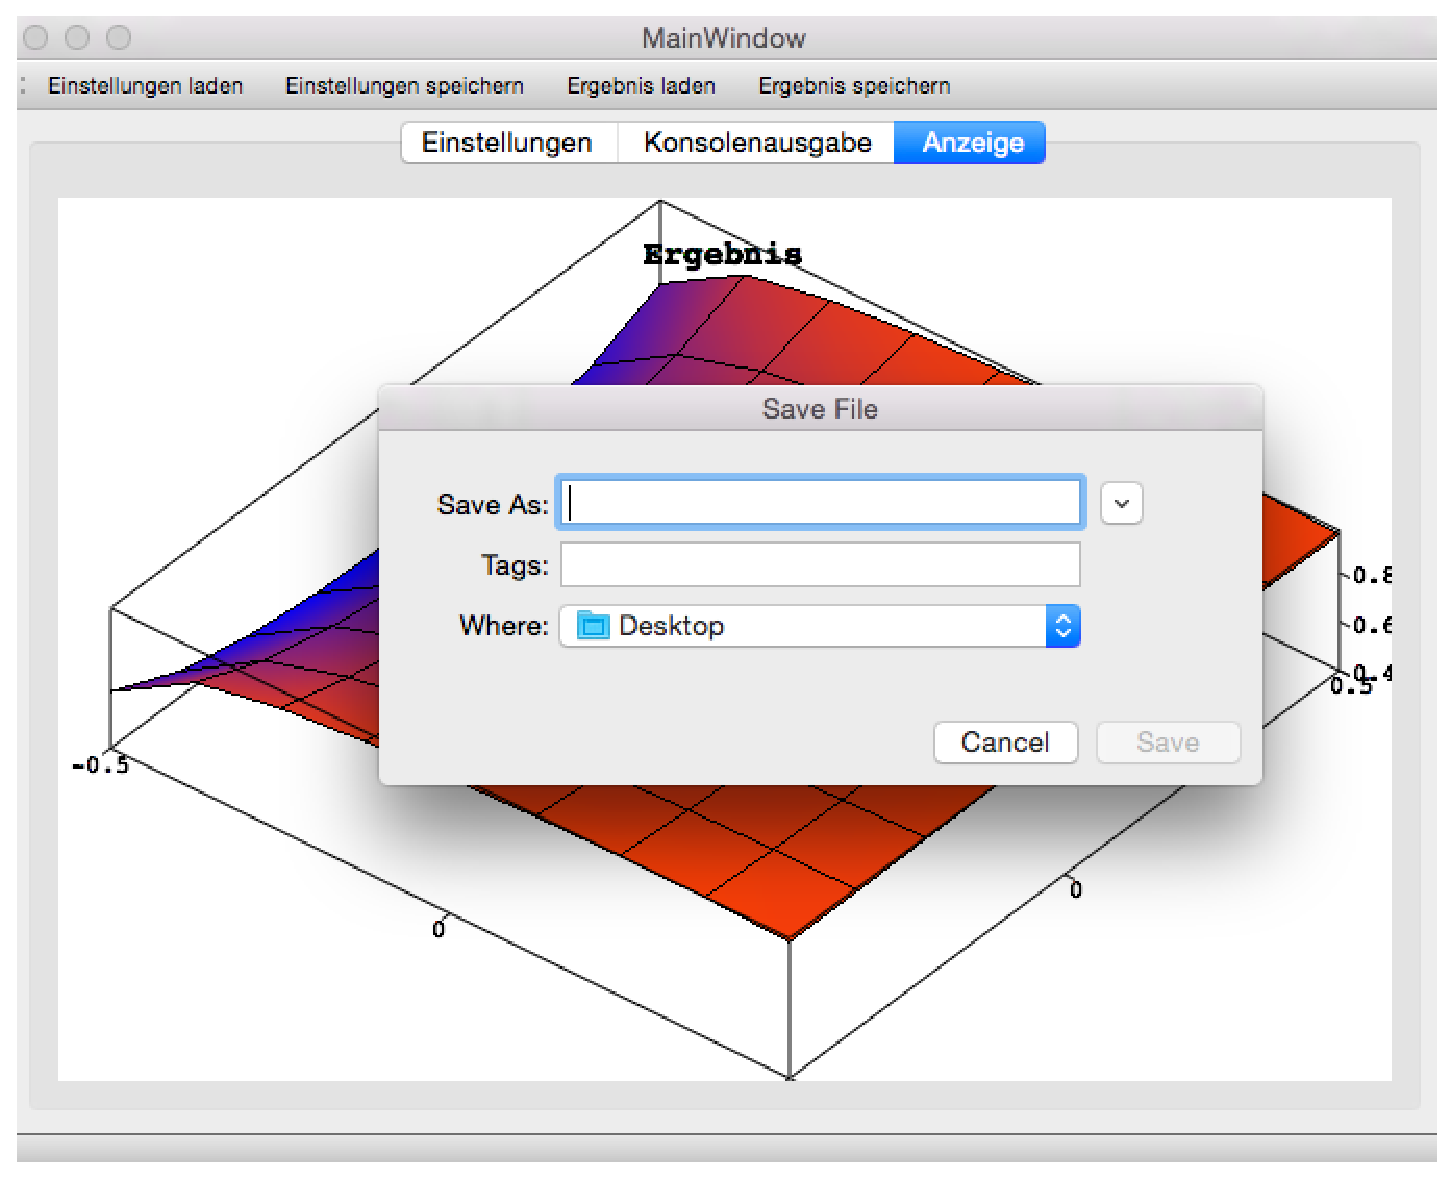
\epsfig{file=nutzerdoc/Ergebnis_Speichern.eps,width=\textwidth}
% Bild Ergebnis_Speichiern.png
\subsection{Ergebnis laden}
Nachdem der Nutzer den Button "'Ergebnis laden" geklickt hat, erscheint ein Dialogfenster, wo der Nutzer das Verzeichnis suchen kann, wo sich die Datei im \textbf{.surface}-Format befinet. Durch anschlie\ss endes Klicken auf den Open-Button werden die Ergebnisse geladen und die Minimalfl\"ache angezeigt. \newline
% Bild Ergebnis_Laden.png 
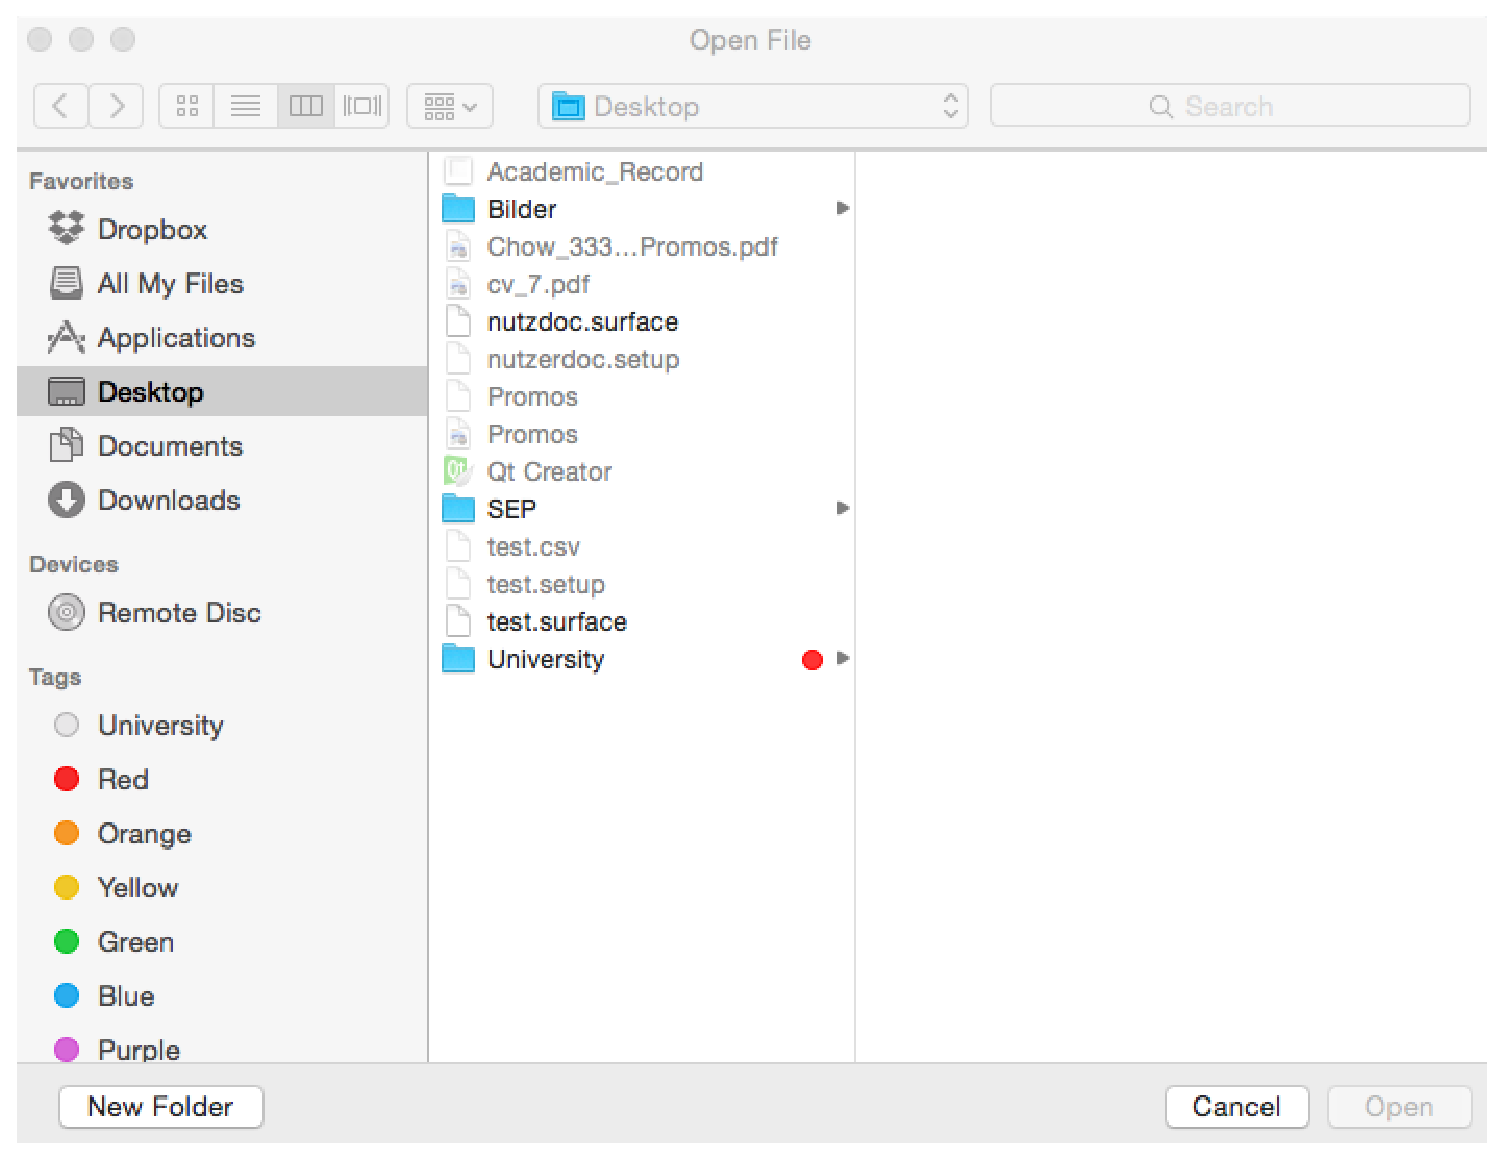
\epsfig{file=nutzerdoc/Ergebnis_Laden.eps,width=\textwidth}

\subsection{Mit der .surface-Datei weiterarbeiten}
In diesem Abschnitt wird eine kurz Einf\"uhrung gegeben, wie man mit einer .surface-Datei in  \"ublichen Datenanalyseprogrammen weiterarbeiten kann. Als Beispiel wird hierf\"ur \textbf{MATLAB} genommen. \\
%% Bild Matlaboberfl�che
\epsfig{file=nutzerdoc/3.eps,width=\textwidth}
\\ 
Nachdem man auf \textit{Import Data} geklickt hat, muss man bei den Dateientypen \textbf{All files} ausw\"ahlen, damit die .surface-Dateien zur Auswahl angezeigt werden kann. In unserem Fall importieren wir die Daten aus der Datei \textit{standard.surface}. Nachdem man die zu ausgewerteten Daten markiert hat und die Importeinstellung \textit{Numeric Matrix} ausgew\"ahlt ist, kann man unter \textit{Import Selection} die Unterfunktion \textit{Generate Script} anklicken.
\\
\epsfig{file=nutzerdoc/1.eps,width=\textwidth}
\\
Nun werden die Daten in Matlab geladen, welche z.B. mit dem Befehl \textbf{surf(filename)} geplottet werden k\"onnen.
\\
\epsfig{file=nutzerdoc/tier1.eps,width=\textwidth}
\\
\section{Eingaben}
Das Programm besitzt zwar eingebaute Erkennung richtiger Eingabewerte, jedoch nicht Erkennung sinnvoller Eingabewerte, d.h. wie sich die Rechenzeit in Abh\"angigkeit der eingegebenen Parameter verh\"alt. Im Folgenden sind also Wertebereiche beschrieben, bei denen das Programm nicht l\"anger als eine Minute Laufzeit auf einem durchschnittlichen Laptop hatte. 
\begin{itemize}
  \item $ \epsilon \in [10^{-9},1] $
  \item $ iterations \in [10,20] $
  \item $ stuetz_x, stuetz_y \in [10,60] $
\end{itemize}
Am gr\"o\ss ten beeinflusst wird die Laufzeit des Programms durch die gew\"ahlte Anzahl der St\"utzstellen. \\
Die Wahl der Randfunktionen ist relativ beliebig und gut gesch\"utzt, d.h. durch Fehlersituationen abgefangen. Ebenso beliebig ist die Wahl des Definitionsbereichs, welche auch durch entsprechende Fehlermeldungen gesch\"utzt ist. \\
Weiterhin werden die Randfunktionen nur auf ihre Syntaktische Korrektheit �berpr�ft und nicht auf m\"ogliche Singularit\"aten oder Divisionen durch Null. Dies kann ein Grund f\"ur Divergenz des L\"osers sein.
Deshalb sollte beachtet werden, dass keine Kovergenz, bzw. kein sinnvolles Ergebnis, f�r das vom Benutzer gestellten Problems garantiert wird.

\section{Beispielsitzung}
Nun wird eine Beispielsitzung in dem Programm durchgef\"uhrt. In der Sitzung werden zwei Berechnungen ausgef\"uhrt, Einstellungen geladen und Ergebnisse gespeichert.
Zun\"achst jedoch wird das Programm gestartet.

\begin{figure}[H]
\centering
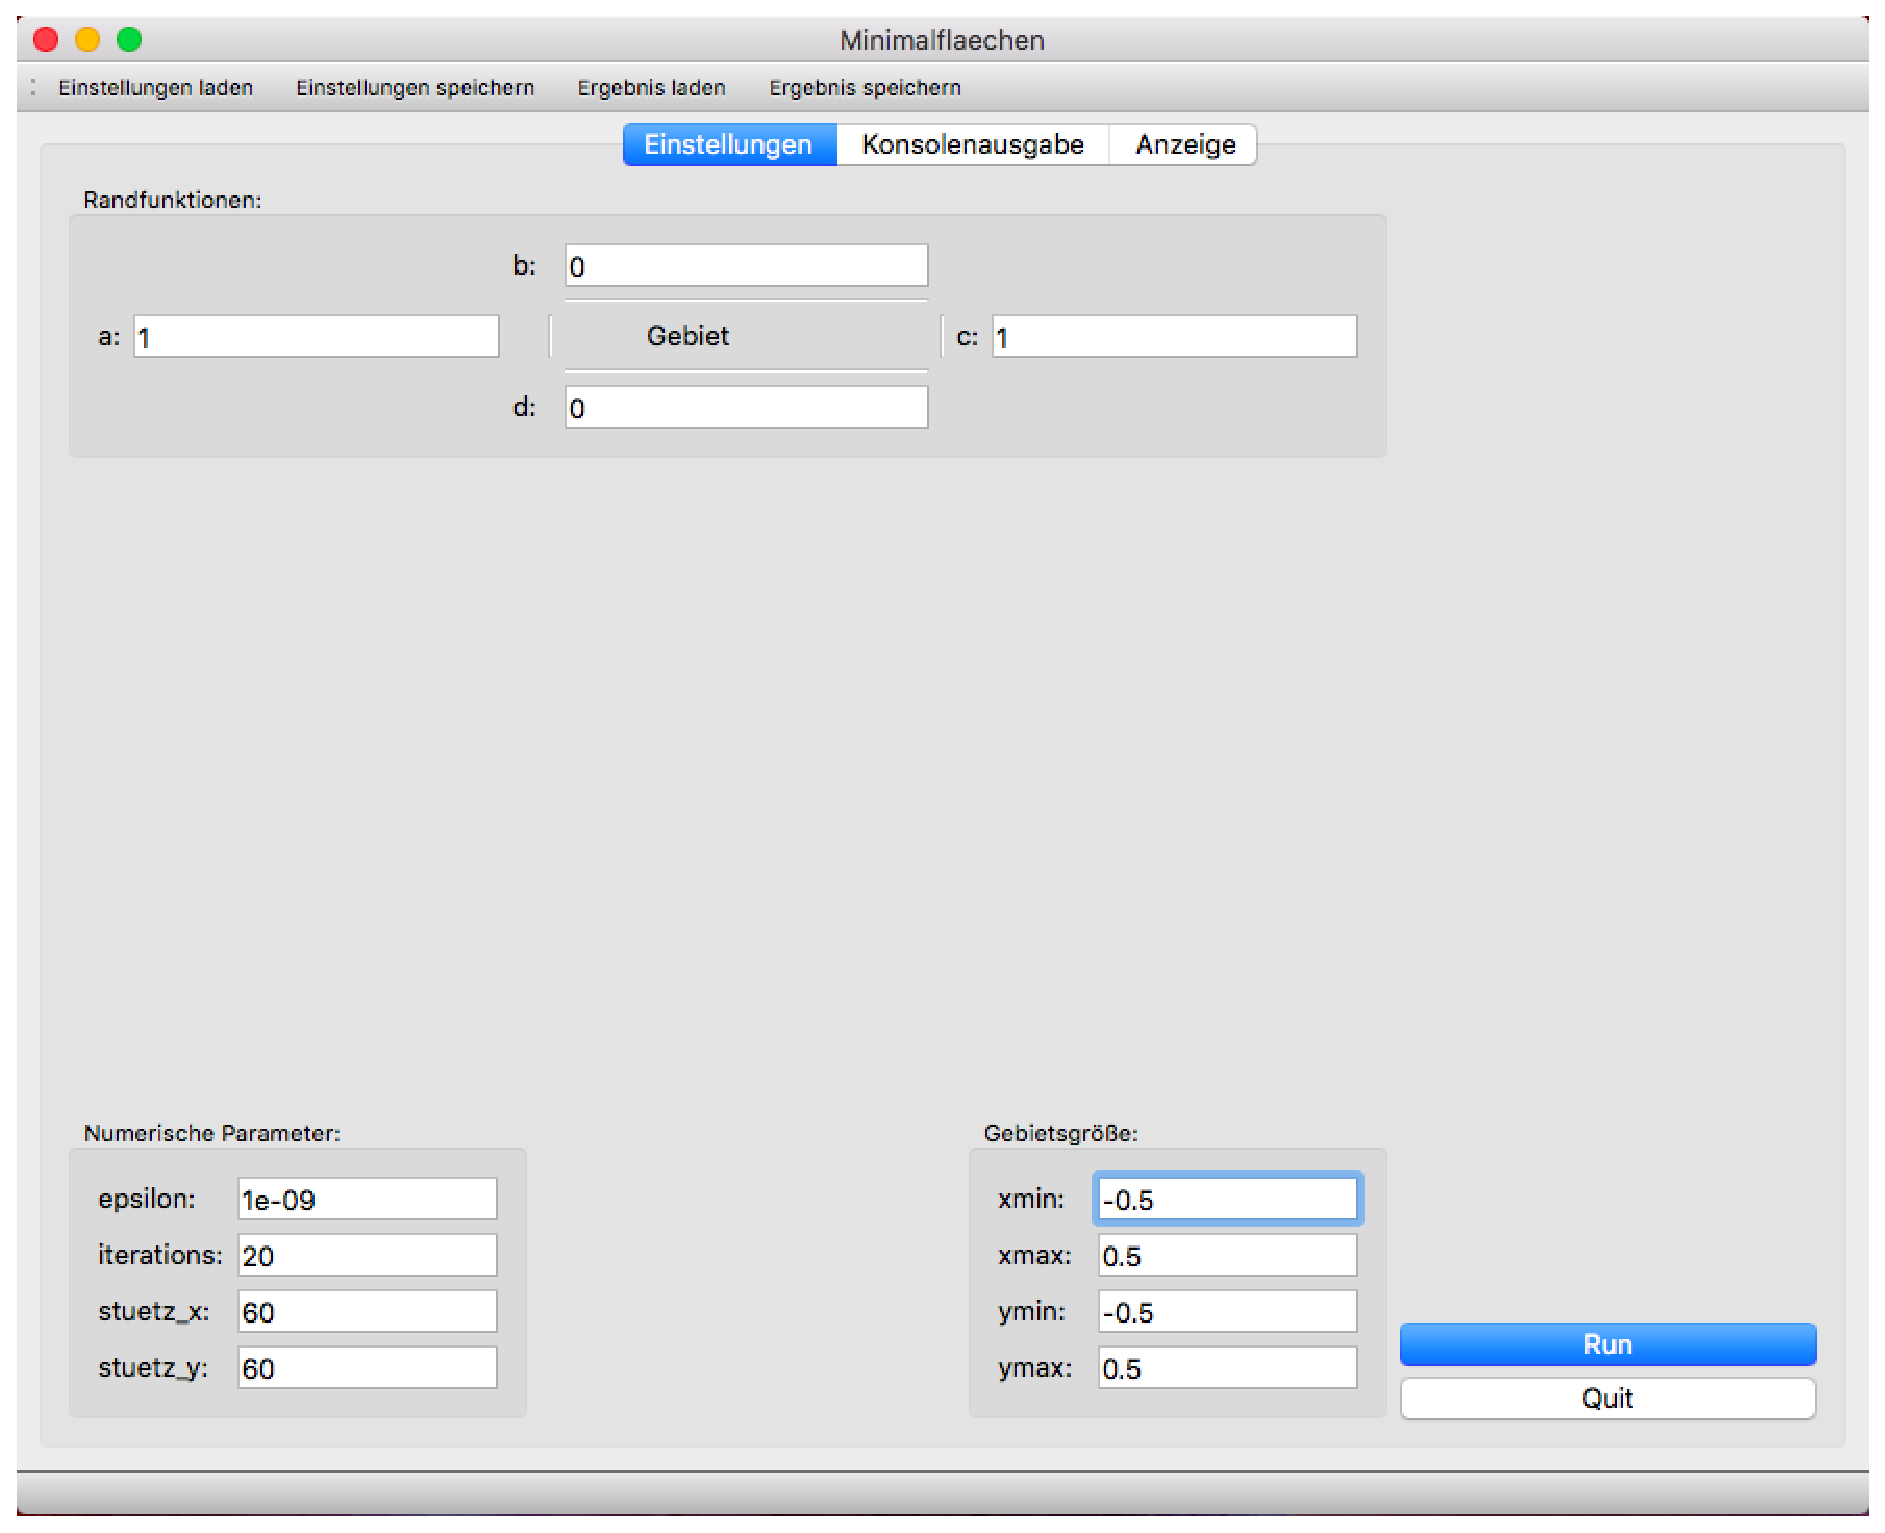
\includegraphics[width=\textwidth]{nutzerdoc/example_session/bsp_1}
\caption{Startbildschirm des Programms}
\end{figure}

In dem Startbildschirm k\"onnen alle relevanten Einstellungen f\"ur die Berechnung der Minimalfl\"ache festgelegt werden. In diesem Beispiel wird jedoch direkt auf den {\tt run} Button geklickt. Dies wechselt die Ansicht auf den mittleren Tab {\tt Konsolenausgabe}.

\begin{figure}[H]
\centering
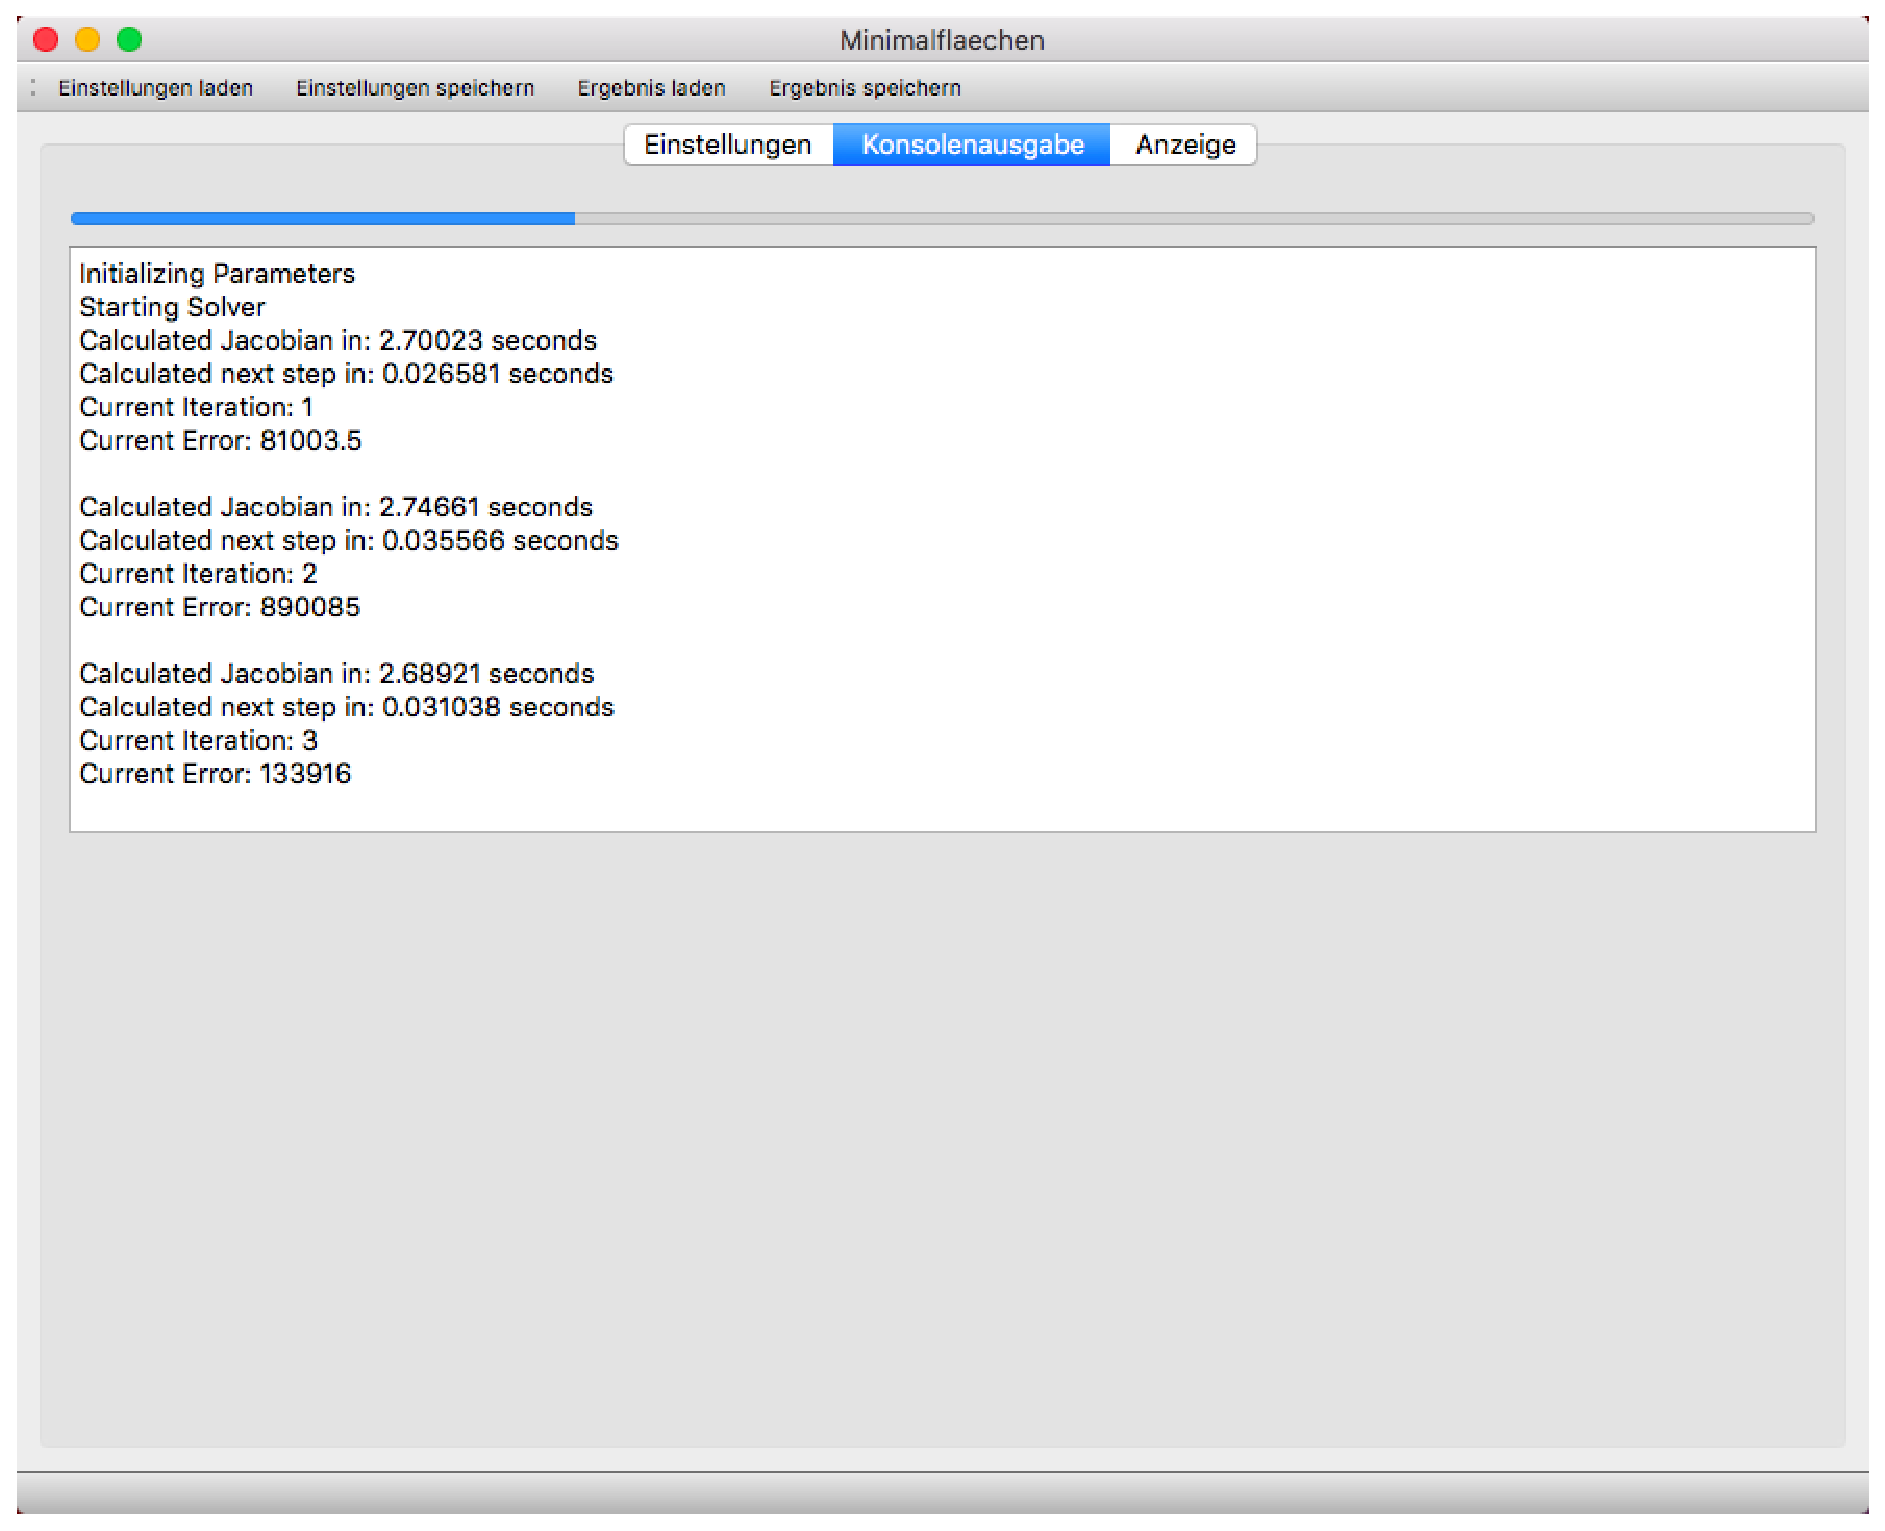
\includegraphics[width=\textwidth]{nutzerdoc/example_session/bsp_2}
\caption{Startbildschirm des Programms}
\end{figure}

Hier ist der aktuelle Berechnungsfortschritt zu sehen, sowie der Konvergenzfehler und ben\"otigte Zeit der einzelnen Iterationen. Am Ende der Berechnung ist hier auch zu sehen, ob die Problemstellung zu dem gew\"unschten Fehler konvergiert ist. Nun wird auf den {\tt Anzeige} Tab gewechselt. 

\begin{figure}[H]
\centering
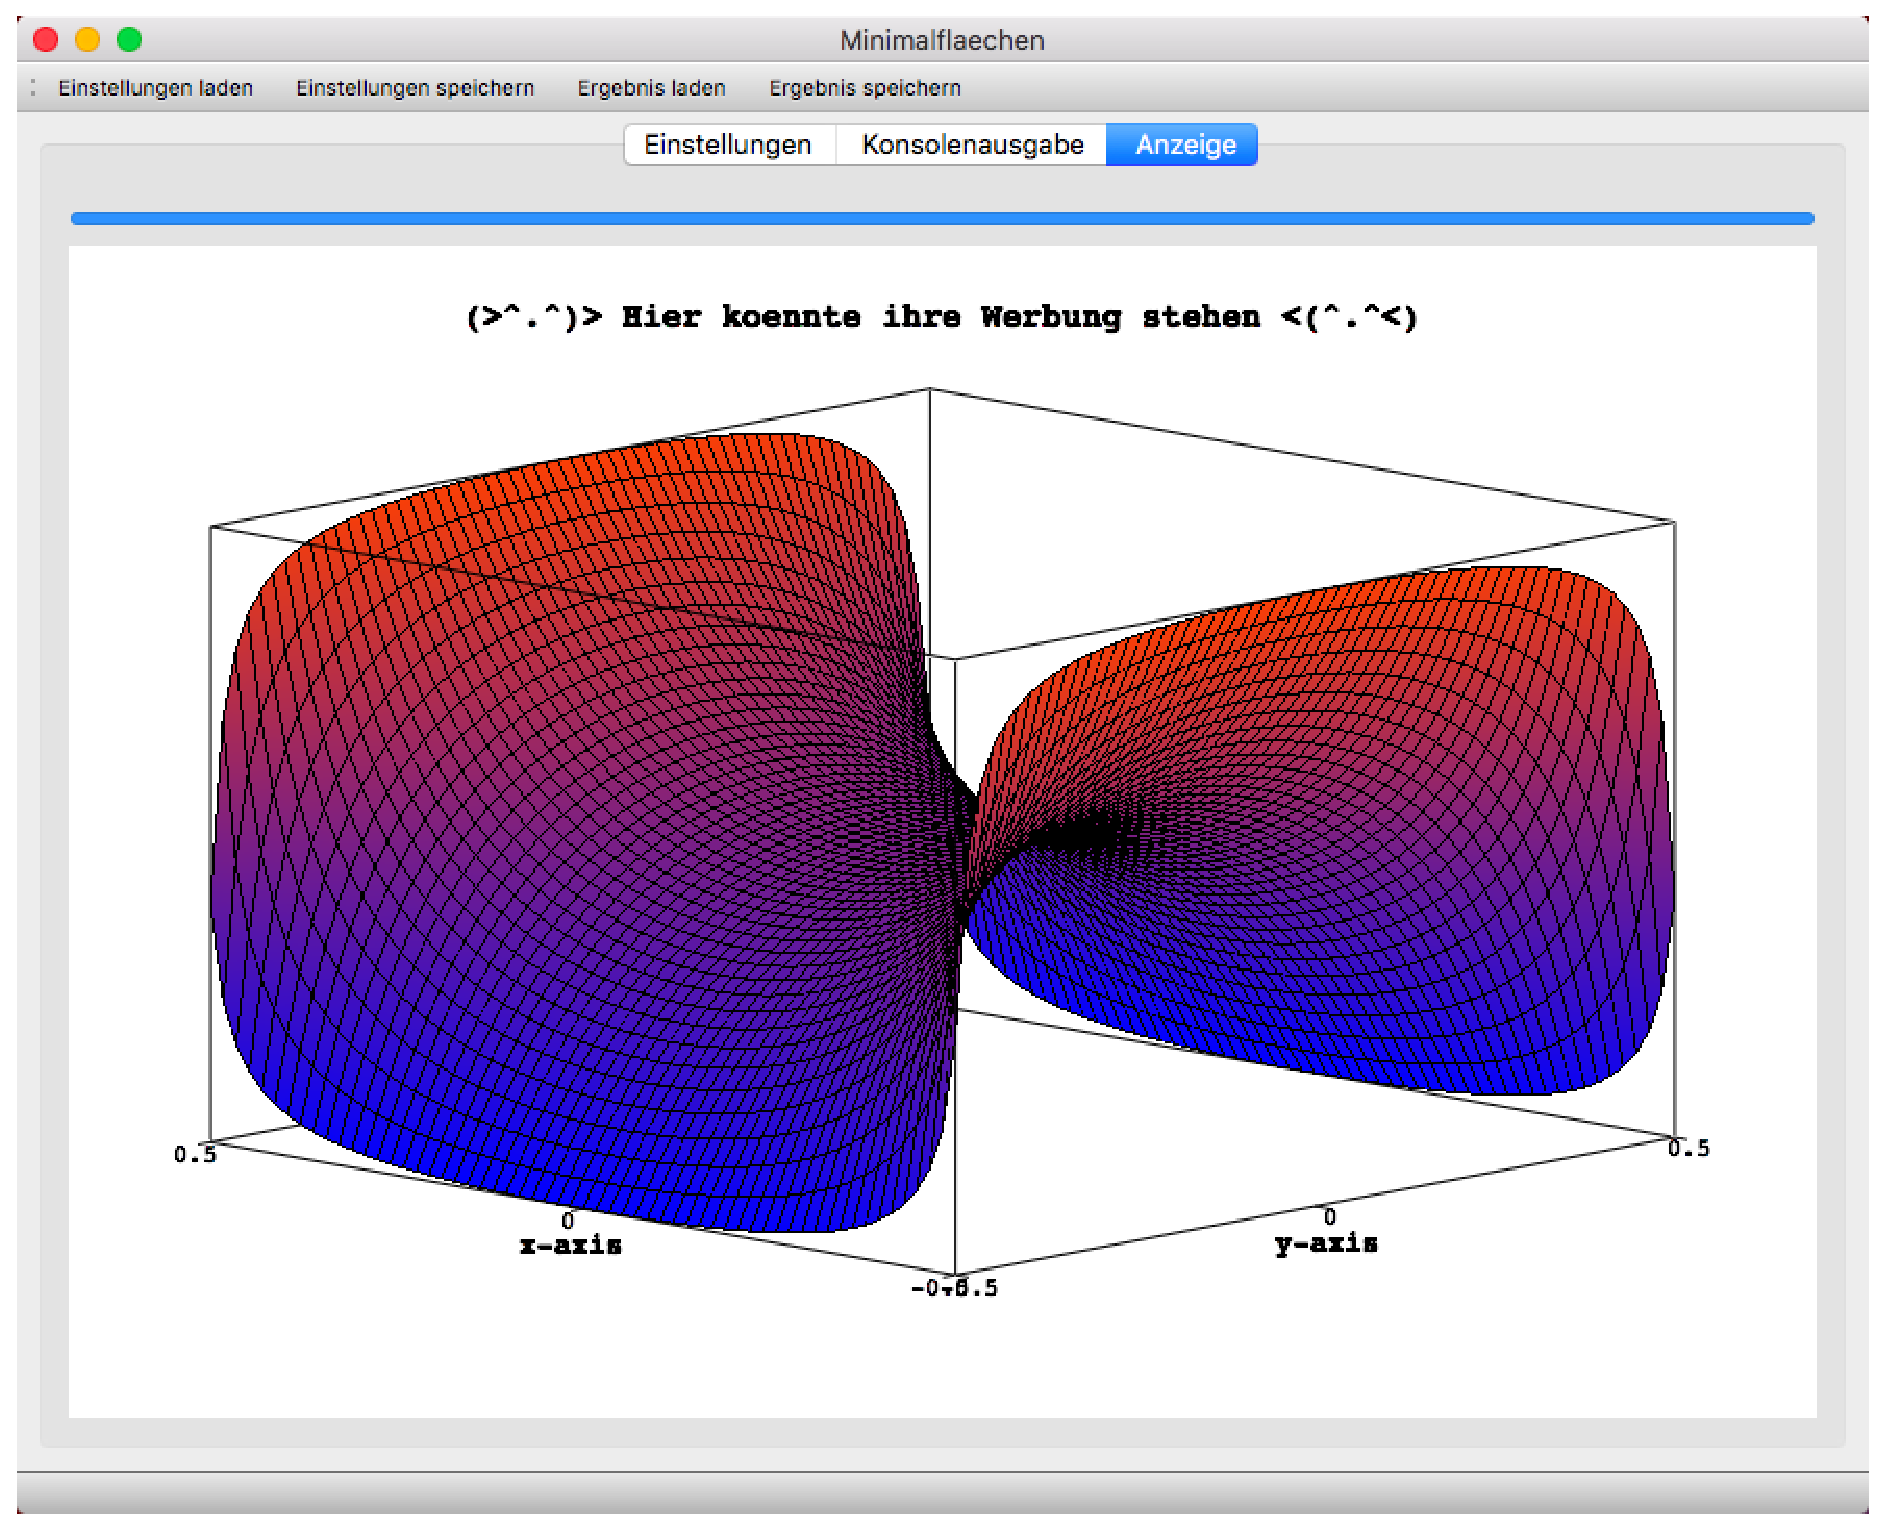
\includegraphics[width=\textwidth]{nutzerdoc/example_session/bsp_3}
\caption{Startbildschirm des Programms}
\end{figure}

Hier wird das Ergebnis der Berechnung angezeigt. Es kann ganz intuitiv in das Ergebnis geklickt werden, um die Fl\"ache z.B. zu Rotieren oder Skalieren. Da dieses Ergebnis keine wirkliche Relevanz hat, wird es dieses Mal nicht gespeichert. Anstelle dessen werden die Einstellung des Referenzproblems geladen.

\begin{figure}[H]
\centering
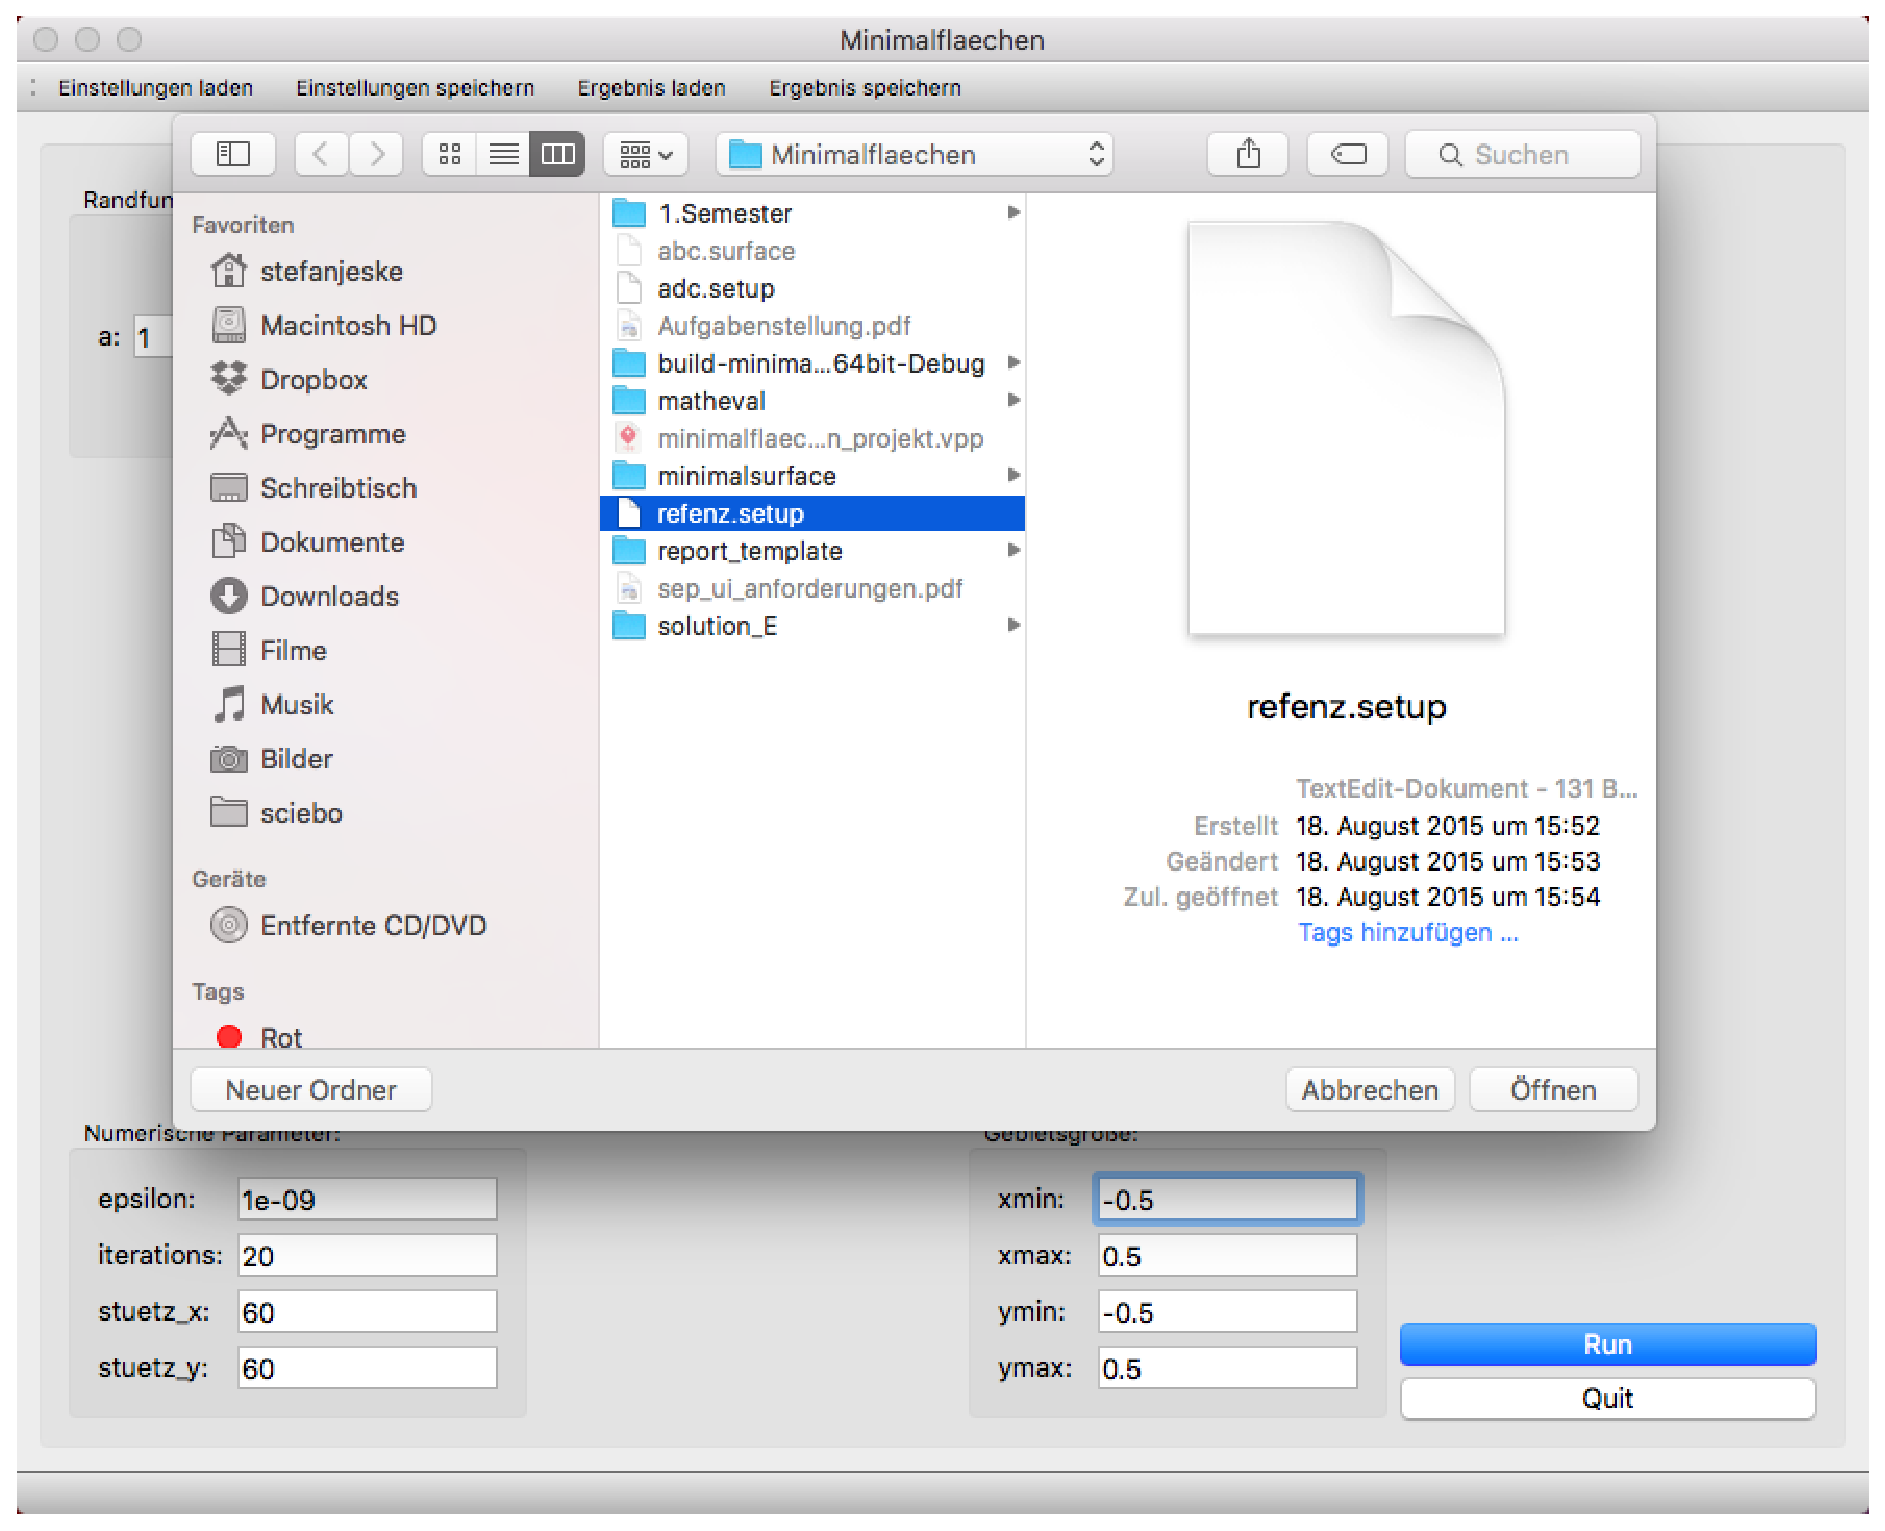
\includegraphics[width=\textwidth]{nutzerdoc/example_session/bsp_4}
\caption{Startbildschirm des Programms}
\end{figure}

Dazu wird auf die Schaltfl\"ache {\tt Einstellungen laden} geklickt und die Datei {\tt referenz.setup} ausgew\"ahlt. Anschlie\ss end wird auf \"offnen geklickt, wodurch die Einstellungen in das Programm geladen werden.

\begin{figure}[H]
\centering
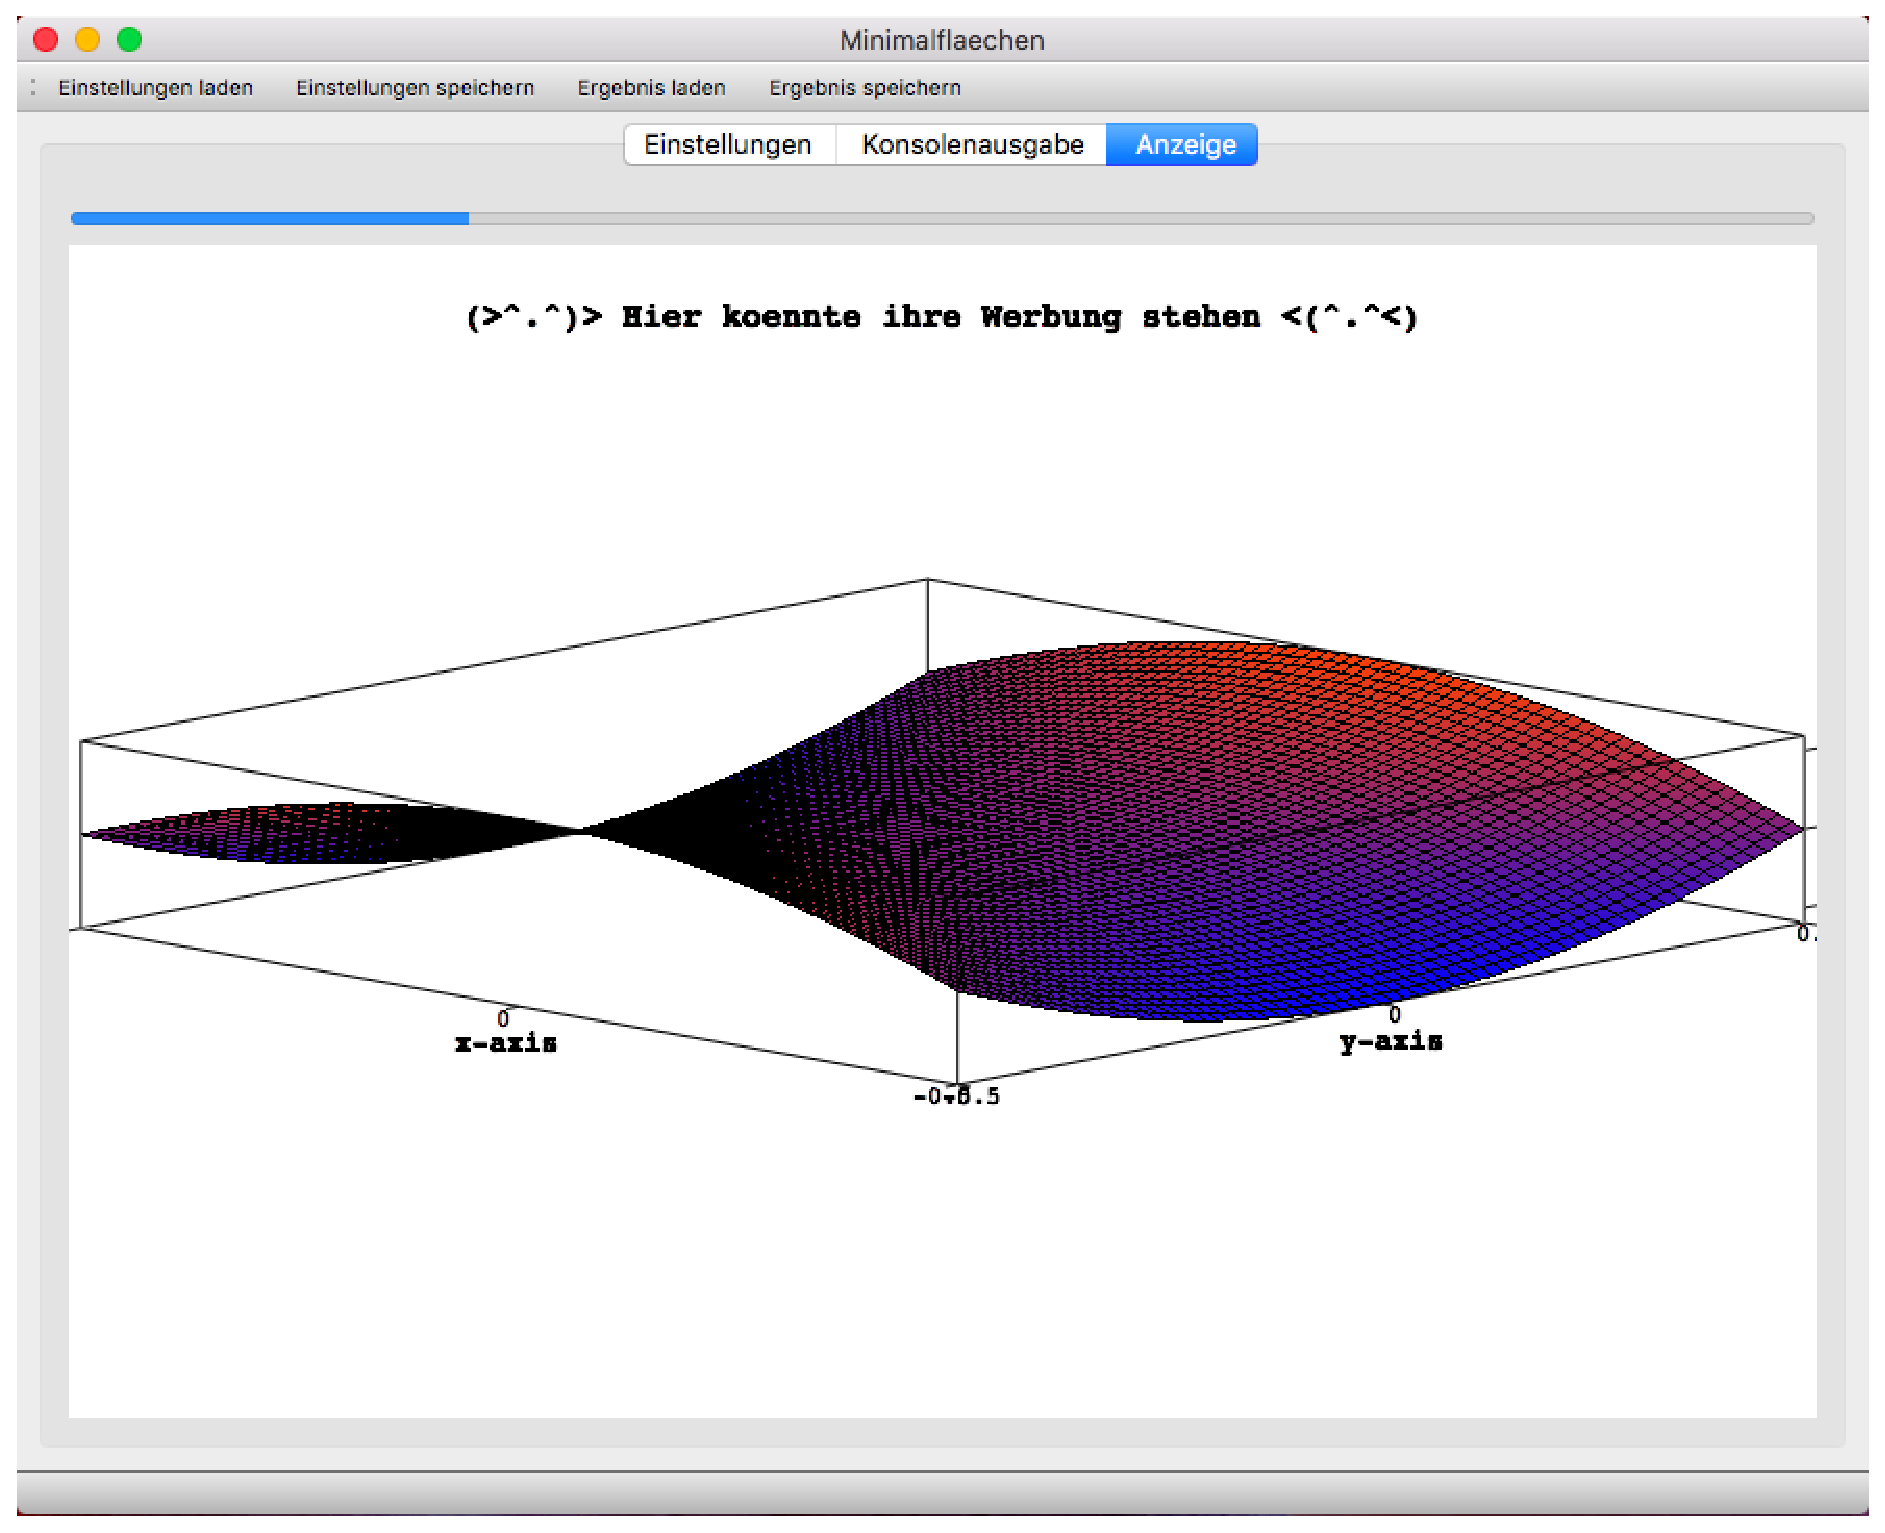
\includegraphics[width=\textwidth]{nutzerdoc/example_session/bsp_5}
\caption{Startbildschirm des Programms}
\end{figure}

Erneut wird auf den {\tt Run} Button geklickt, sodass die Berechnung gestartet wird. Jedoch anstelle wird direkt auf den Tab {\tt Anzeige} gewechselt, um die Entwicklung der Minimalfl\"ache in Echtzeit mitzuvervolgen. Wenn der Fortschrittsbalken voll ist, ist die Berechnung fertig. F\"ur Konvergenz und Rechenzeit kann der {\tt Konsolenausgabe} Tab ge\"offnet werden. Nun wollen wir dieses Ergebnis speichern.

\begin{figure}[H]
\centering
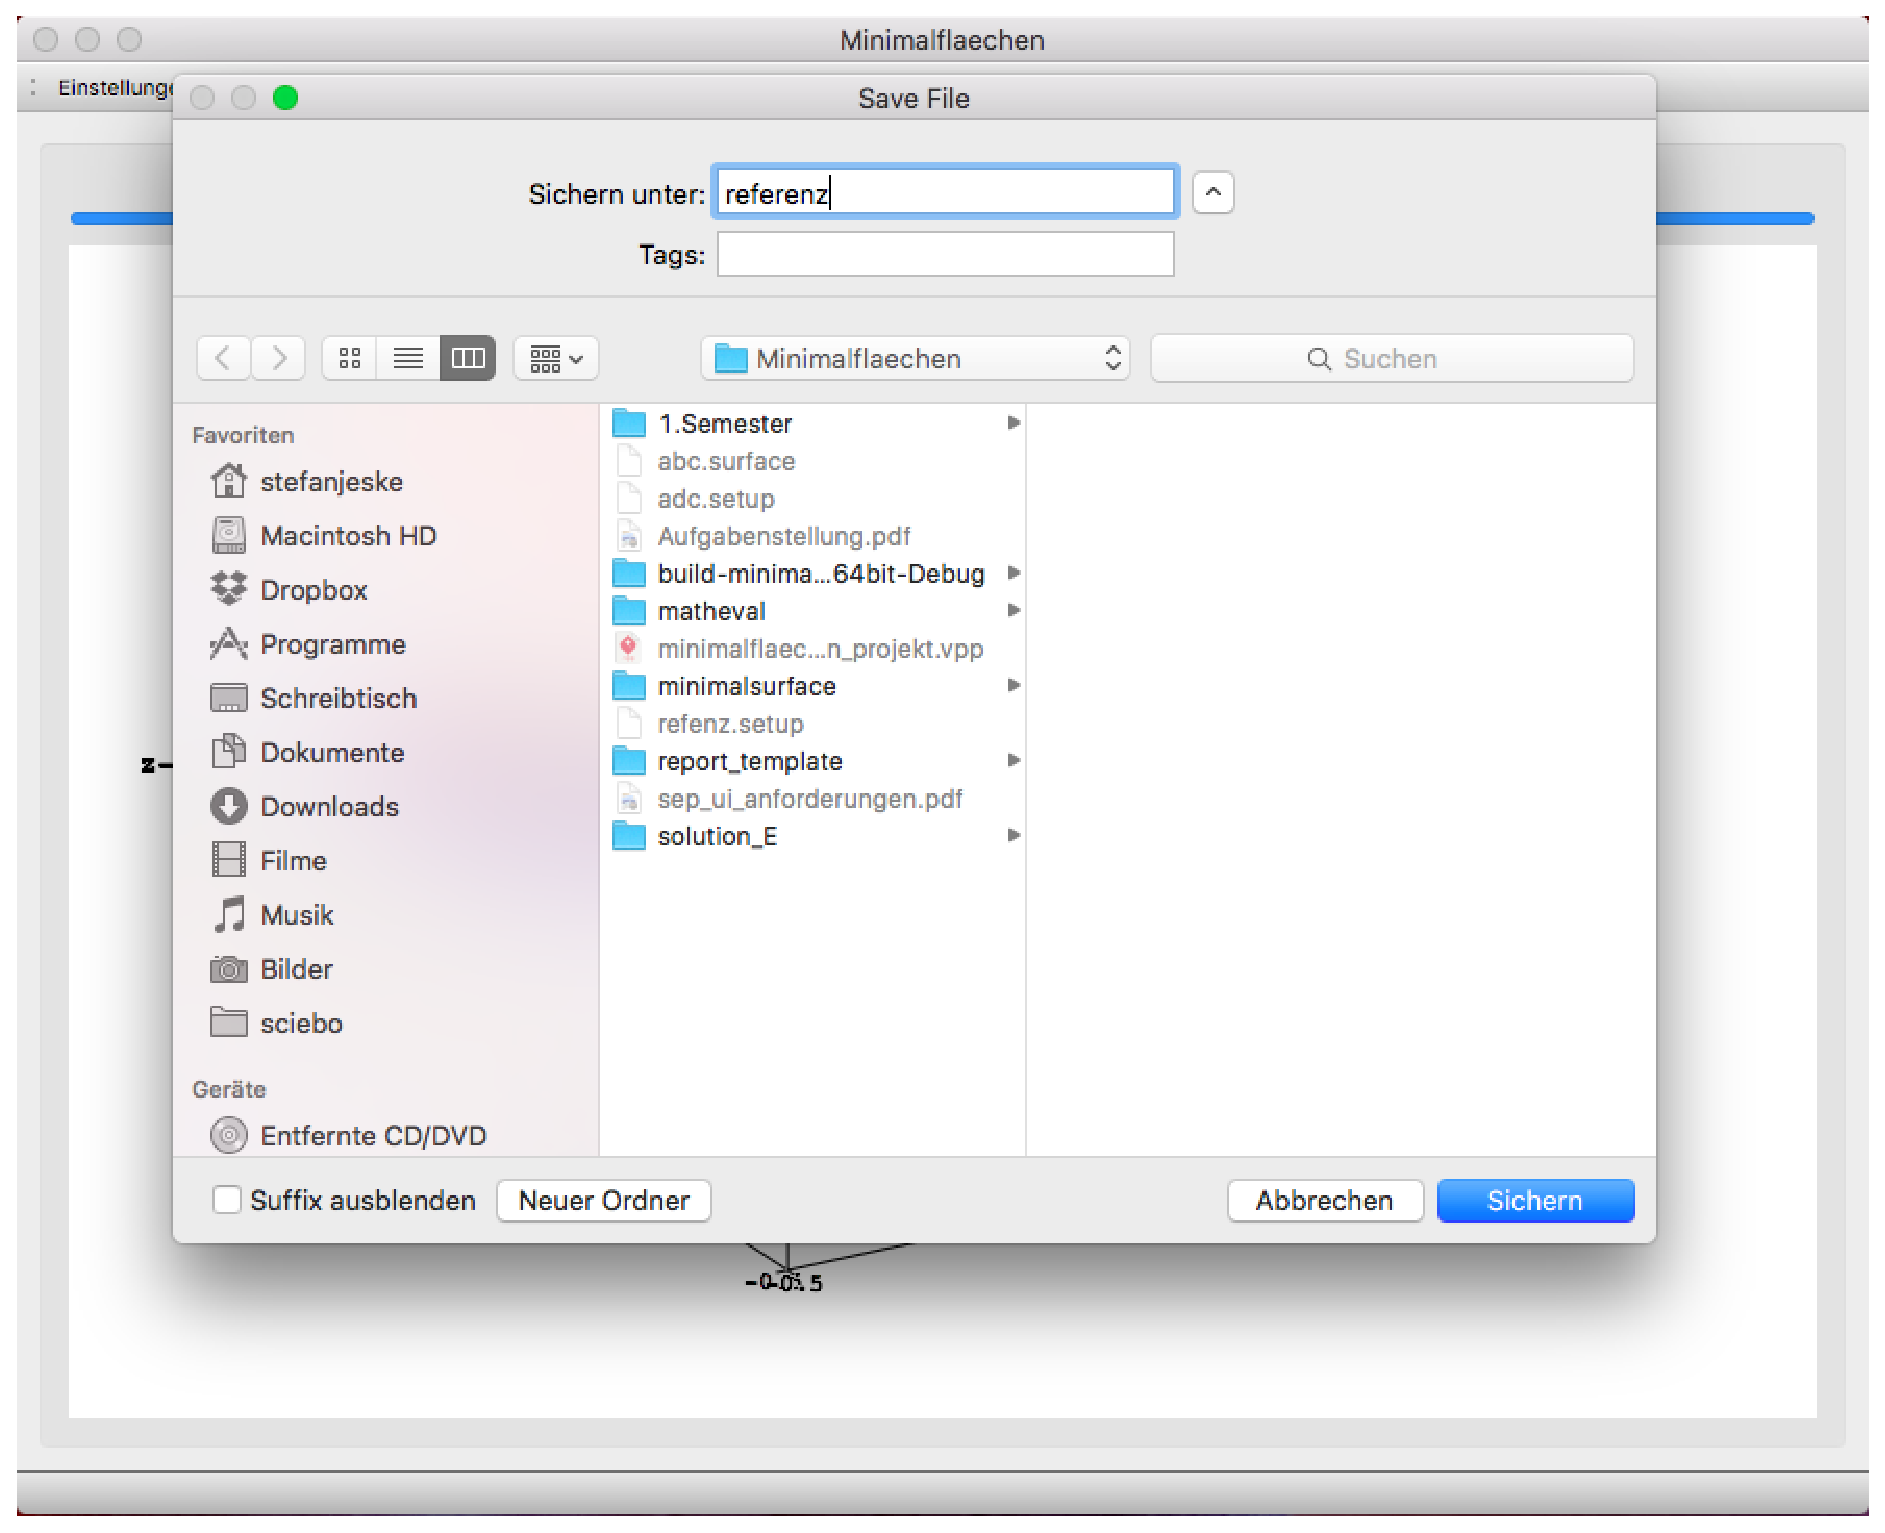
\includegraphics[width=\textwidth]{nutzerdoc/example_session/bsp_6}
\caption{Startbildschirm des Programms}
\end{figure}

Es wird der gew\"unschte Ordner zum Speichern ausgew\"ahlt und der Datei ein Name gegeben. Anschlie\ss end wird auf {\tt Sichern} geklickt, wodurch die berechneten Ergebnisse zur Weiterverwendung bereitstehen. \\
Abschlie\ss end wird das Programm durch Klicken auf den Button {\tt Quit} in dem {\tt Einstellungen} Tab beendet.

\section{Fehlersituationen}
Das Programm gibt Fehlermeldungen aus. Diese werden lediglich durch Fehler in den eingegebenen Funktionen, und durch ung�ltige Definitionsbereichsgrenzen hervorgerufen. \\
Funktionen erzeugen Fehler wenn sie nicht syntaktisch korrekt eingegeben werden, z.B. {\tt lug(x)} anstelle {\tt log(x)}.\\
F\"ur die Definitionsbereichsgrenzen muss lediglich gelten, dass die untere Grenze kleiner ist als die obere.\\
Sollten dennoch Fehler auftreten bitten wir diese an stefan.jeske@rwth-aachen.de zu melden. 